\chapter{CONDUCCIÓN NO PERMANENTE O TRANSITORIA}

\section{Ecuación de \emph{Fourier}}
\begin{equation}
    \frac{\partial^{2}t}{\partial x^2}
    +\frac{\partial^{2}t}{\partial y^2}
    +\frac{\partial^{2}t}{\partial z^2}
    =\frac{1}{\alpha}\,\frac{\partial t}{\partial\theta}
    \label{fourier}
\end{equation}

Pueden resolverse tres tipos de problemas:

\begin{itemize}
    \item Hallar la temperatura: $t=f(x,y,z,\theta)$.
    \item Hallar las coordenadas: $x,y,z=f(t,\theta)$.
    \item Hallar el tiempo: $\theta=f(x,y,z,t)$.
\end{itemize}

\subsection{Distribución de temperaturas en la sección de un cuerpo}

\begin{figure}[!h]
\centering
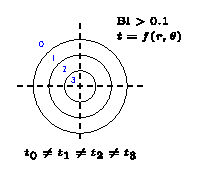
\includegraphics[scale=1.75]{figura03_01.eps}
\caption{Distribución de temperaturas estratificado.}
\end{figure}
\begin{figure}[!h]
\centering
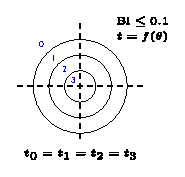
\includegraphics[scale=1.75]{figura03_02.eps}
\caption{Distribución de temperaturas uniforme.}
\end{figure}

\section{Número de \emph{Biot} (Bi)}
Deducción:
\begin{figure}[!h]
\centering
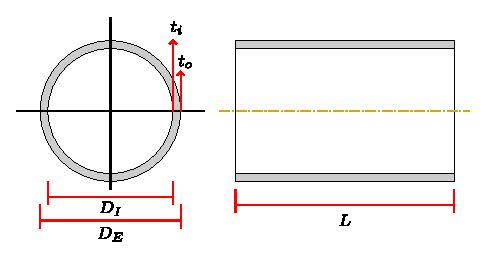
\includegraphics[scale=1.25]{figura03_03.eps}
\caption{Cilindro de pared delgada.}
\end{figure}

\begin{equation*}
    \text{Bi} = \frac{\text{Resistencia interna}}{\text{Resistencia externa}}
\end{equation*}

Resistencia interna:
\begin{equation*}
    q_{\,\text{conducción}} = k\,A_I\frac{(t_i-t_o)}{\Delta r}
                            = \frac{t_i-t_o}{\frac{\Delta r}{k\,A_I}}
\end{equation*}
\begin{equation*}
    R_I = \frac{\Delta r}{k\,A_I}
\end{equation*}

Resistencia externa:
\begin{equation*}
    q_{\,\text{convección}} = h\,A_E(t_i-t_o)
                            = \frac{t_i-t_o}{\frac{1}{h\,A_E}}
\end{equation*}
\begin{equation*}
    R_E = \frac{1}{h\,A_E}
\end{equation*}

\begin{equation*}
    \text{Bi} = \frac{\frac{\Delta r}{k\,A_I}}{\frac{1}{h\,A_E}}
              = \frac{h\,A_E\,\Delta r}{k\,A_I}
\end{equation*}

Considerando $A_I\approx A_E$:
\begin{equation*}
    \text{Bi} = \frac{h\,\Delta r}{k}
\end{equation*}

Generalizando para cualquier geometría:
\begin{equation}
    \text{Bi} = \frac{h\,L}{k}
\end{equation}

Donde $L$ es la longitud característica:
\begin{equation}
    L = \frac{V}{A}
\end{equation}

\subsection{Resolución de problemas}
Dependiendo del número de \emph{Biot} existen varios métodos de resolución de
problemas:

\begin{itemize}
    \item Caso: $Bi\leq 0.1$ (Distribución de temperatura uniforme)
        \begin{itemize}
            \item Método analítico.
        \end{itemize}
    \item Caso: $Bi>0.1$ (Distribución de temperatura estratificada)
        \begin{itemize}
            \item Método analítico especial.
            \item Método analítico-gráfico.
            \item Método gráfico.
            \item Método de la tabla numérica.
        \end{itemize}
\end{itemize}

\section{Caso: $Bi\leq 0.1$}
\subsection{Método analítico}
\underline{Deducción}:
\begin{figure}[!h]
\centering
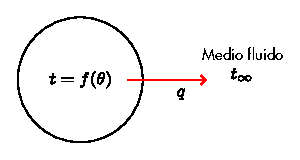
\includegraphics[scale=1.25]{figura03_04.eps}
\end{figure}
\begin{equation*}
    t > t_{\infty}
\end{equation*}
\begin{equation*}
    \theta = f(t)
\end{equation*}

\textbf{Balance de energía}: Calor transmitido por convección al medio fluido
= Disminución del calor sensible del cuerpo.
\begin{equation*}
    h\,A\,(t-t_{\infty}) = -m\,C_p\,\frac{dt}{d\theta}
\end{equation*}
\begin{equation*}
    d\theta = -\frac{m\,C_p\,dt}{h\,A\,(t-t_{\infty})}
\end{equation*}

Se asumen constantes: $m$, $h$, $A$ y $C_p$.
\begin{equation*}
    \int_t \frac{dt}{t-t_{\infty}} =
    \frac{h\,A}{m\,C_p}\,\int_0^{\theta} d\theta
\end{equation*}
\begin{equation*}
    -\ln\left(\frac{t_i-t_{\infty}}{t_f-t_{\infty}}\right) =
    \frac{h\,A}{m\,C_p}\,\theta
\end{equation*}
\begin{equation*}
    \theta =
    -\frac{m\,C_p}{h\,A}\,\ln\left(\frac{t_f-t_{\infty}}{t_i-t_{\infty}}\right)
    \label{uniforme_tiempo}
\end{equation*}

Asumiendo $t_f=t$:
\begin{equation}
    \theta = f(\theta) =
    -\frac{m\,C_p}{h\,A}\,\ln\left(\frac{t_f-t_{\infty}}{t_i-t_{\infty}}\right)
\end{equation}

\begin{equation*}
    \ln\left(\frac{t_f-t_{\infty}}{t_i-t_{\infty}}\right) =
    -\frac{h\,A\,\theta}{m\,C_p}
\end{equation*}
\begin{equation}
    \frac{t_f-t_{\infty}}{t_i-t_{\infty}} =
    e^{-\dfrac{h\,A\,\theta}{m\,C_p}}
    \label{uniforme_temperatura1}
\end{equation}

El exponente puede presentarse de otro modo:
\begin{equation*}
    \frac{h\,A\,\theta}{m\,C_p}
\end{equation*}

Sabiendo que $\rho=m/V$:
\begin{equation*}
    \frac{h\,A\,\theta}{\rho\,V\,C_p}
\end{equation*}

Sabiendo que $V=A\,L$:
\begin{equation*}
    \frac{h\,\theta}{\rho\,L\,C_p}
\end{equation*}

Sabiendo que $\alpha=k/\rho\,C_p$:
\begin{equation*}
    \frac{\alpha\,h\,\theta}{k\,L}
\end{equation*}

Multiplicando por $L/L$:
\begin{equation*}
    \frac{h\,L\,\alpha\,\theta}{k\,L^2} =
    \left(\frac{h\,L}{k}\right)\left(\frac{\alpha\,\theta}{L^2}\right)
\end{equation*}

Se define el número de \emph{Biot}, como:
\begin{equation*}
    \text{Bi} = \frac{h\,L}{k}
\end{equation*}

Se define el número de \emph{Fourier}, como:
\begin{equation}
    \text{Fo} = \frac{\alpha\,\theta}{L^2}
\end{equation}

Por tanto la ecuación (\ref{uniforme_temperatura1}) puede definirse como:
\begin{equation}
    \frac{t-t_{\infty}}{t_i-t_{\infty}} = e^{-\text{Bi}\,\text{Fo}}
    \label{uniforme_temperatura2}
\end{equation}

\section{Caso: $Bi>0.1$}

\subsection{Método analítico especial}
Se aplica para el caso de una placa de área infinita y resistencia superficial
igual a $0$ o $h=\infty$.

\begin{figure}[!h]
\centering
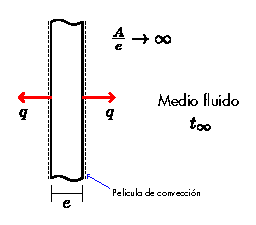
\includegraphics[scale=1.75]{figura03_05.eps}
\end{figure}
\begin{equation*}
    q = h\,A\,\Delta t = \dfrac{\Delta t}{\frac{1}{h\,A}}
\end{equation*}

La resistencia térmica es:
\begin{equation*}
    R = \frac{1}{h\,A}
\end{equation*}

La condición necesaria requiere una resistencia $R=0$, es decir:

\begin{equation*}
    A\rightarrow\infty
\end{equation*}
o:
\begin{equation*}
    h\rightarrow\infty
\end{equation*}

\begin{figure}[!h]
\centering
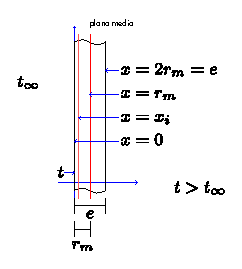
\includegraphics[scale=1.75]{figura03_06.eps}
\end{figure}

Para un flujo unidireccional, se tiene:
\begin{equation*}
    \frac{\partial^2 t}{\partial x^2} =
    \frac{1}{\alpha}\frac{\partial t}{\partial\theta}
\end{equation*}

Cuya solución es:
\begin{equation}
    \frac{t_f-t_\infty}{t_i-t_\infty} = \frac{4}{\pi}\left[
        e^{-a_1 X}\,\sen\left(\frac{\pi x}{2r_m}\right)+
        \frac{1}{3}\,e^{-9a_1 X}\,\sen\left(\frac{3\pi x}{2r_m}\right)+
        \cdots
    \right]
    \label{analitico_especial}
\end{equation}

Donde:
\begin{equation}
    a_1 = \left(\frac{\pi}{2}\right)^2
\end{equation}
\begin{equation}
    X = \frac{\alpha\,\theta}{r_m^2}
\end{equation}

Esta es una serie infinita, que converge rápidamente, por lo que usar los dos
primeros términos son suficientes.

La solución para problemas tipo $t = f(x,\theta)$ es directa, al ser la variable
$t$ fácilmente despejable.

Sin embargo, para problemas tipo $x = f(t,\theta)$ y $\theta = f(x,t)$, se debe
utilizar un calculo iterativo.

\subsubsection{Calculo iterativo}
Para resolver problemas tipo $x = f(t,\theta)$, se siguen los siguientes pasos:

\begin{enumerate}
    \item Resolvemos x solo con el primer termino.
    \item El valor obtenido de $x$ es una valor de referencia $x_{\text{ref}}$.
    \item Sobre el valor $x_{\text{ref}}$, hacemos variar un poco arriba o hacia
        abajo su valor.
    \item Reemplazamos en los dos términos de la solución y resolvemos el
        segundo termino de la ecuación (\ref{analitico_especial}).
    \item Comparar con el primer termino de la ecuación
        (\ref{analitico_especial}), si ambos valores son iguales el problema
        esta resuelto.
    \item Si los valores son diferentes debe seguir iterándose.
\end{enumerate}

\subsection{Método analítico-gráfico}
Para este método se requieren las siguientes definiciones:

Temperatura relativa:
\begin{equation*}
    y = \frac{t_f-t_\infty}{t_i-t_\infty}
\end{equation*}

Tiempo relativo:
\begin{equation*}
    x = \frac{\alpha\theta}{r_m^2}
\end{equation*}

Resistencia relativa:
\begin{equation*}
    m = \frac{k}{h\,r_m}
\end{equation*}

Posición relativa:
\begin{equation*}
    n = \frac{r}{r_m}
\end{equation*}

\begin{figure}[!h]
\centering
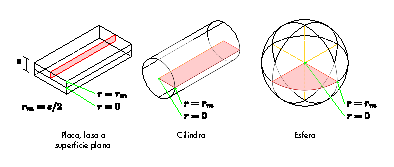
\includegraphics[scale=2.35]{figura03_07.eps}
\end{figure}

Casos de estudio:

\begin{enumerate}
    \item El valor de $x$ no esta en la gráfica.\\
    \textbf{Solución}: Alargar el eje de $x$ y prolongar la linea.
    \item El valor de $m$ no coincide con los valores mostrados en la gráfica.\\
    \textbf{Solución}: Se debe realizar una interpolación gráfica.
    \item No es posible intersecar la linea vertical trazada por $x$.\\
    \textbf{Solución}: No es posible solucionar.
    \item La placa esta expuesta a temperaturas diferentes.\\
    \textbf{Solución}: No es posible, pero se puede resolver con el método
    gráfico.
    \item El valor de $m$ no se encuentra en la gráfica.\\
    \textbf{Solución}: Recurrir a la gráfica de \emph{Ocon} y \emph{Tojo}.
\end{enumerate}

\section{Método gráfico o método de \emph{Schmidt}}

\subsection{Principio de \emph{Dusinberre}}
\begin{figure}[!h]
\centering
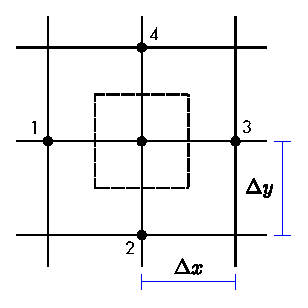
\includegraphics[scale=1.20]{figura03_08.eps}
\end{figure}

Balance de calor en el nodo $0$:
\begin{equation*}
    q_{1\rightarrow 0}+
    q_{2\rightarrow 0}+
    q_{3\rightarrow 0}+
    q_{4\rightarrow 0}=
    q_s
\end{equation*}
\begin{equation*}
    k_x\frac{A_x}{\Delta x}(t_1-t_0)+
    k_y\frac{A_y}{\Delta y}(t_2-t_0)+
    k_x\frac{A_x}{\Delta x}(t_3-t_0)+
    k_y\frac{A_y}{\Delta y}(t_4-t_0)=
    m\,C_p\frac{t_0^{'}-t_0}{\Delta\theta}
\end{equation*}

Donde:
\begin{itemize}
    \item $t_0^{'}$: Nueva temperatura del nodo $0$.
    \item $\Delta\theta$: Incremento de tiempo.
\end{itemize}

Considerando $\Delta x=\Delta y$, $A_x=A_y=A$ y $k_x=k_y=k$:
\begin{equation*}
    (t_1-t_0)+
    (t_2-t_0)+
    (t_3-t_0)+
    (t_4-t_0)=
    \frac{m\,C_p}{\Delta\theta}\frac{\Delta x}{k\,A}(t_0^{'}-t_0)
\end{equation*}

Considerando $\rho=m/V$:
\begin{equation*}
    \frac{m\,C_p}{\Delta\theta}\frac{\Delta x}{k\,A}=
    \frac{\rho\,V\,C_p}{\Delta\theta}\frac{\Delta x}{k\,A}=
    \frac{\rho\,A\,\Delta x\,C_p}{\Delta\theta}\frac{\Delta x}{k\,A}=
    \frac{\rho\,C_p}{\Delta\theta}\frac{\Delta x^2}{k}
\end{equation*}

Considerando $\alpha=k/\rho\,C_p$:
\begin{equation*}
    \frac{m\,C_p}{\Delta\theta}\frac{\Delta x}{k\,A}=
    \frac{\Delta x^2}{\alpha\,\Delta\theta}=
    M
\end{equation*}

Por tanto:
\begin{equation*}
    (t_1-t_0)+
    (t_2-t_0)+
    (t_3-t_0)+
    (t_4-t_0)=
    M(t_0^{'}-t_0)
\end{equation*}
\begin{equation*}
    t_1+t_2+t_3+t_4-4t_0=M(t_0^{'}-t_0)
\end{equation*}
\begin{equation*}
    t_1+t_2+t_3+t_4-4t_0=M\,t_0^{'}-M\,t_0
\end{equation*}
\begin{equation*}
    M\,t_0^{'}=t_1+t_2+t_3+t_4-4t_0+M\,t_0
\end{equation*}
\begin{equation}
    t_0^{'}=\frac{t_1+t_2+t_3+t_4+(M-4)t_0}{M}
\end{equation}

El parámetro $M$ presenta los siguientes casos:
\begin{itemize}
    \item $M=2$ para flujo en una dimensión.
    \item $M=4$ para flujo en dos dimensiones.
    \item $M=6$ para flujo en tres dimensiones.
\end{itemize}

Para un flujo bidireccional ($M=4$), se tiene:
\begin{equation*}
    t_0^{'}=\frac{t_1+t_2+t_3+t_4}{4}
\end{equation*}
\begin{equation*}
    \frac{\Delta x^2}{\alpha\Delta\theta}=4
\end{equation*}
\begin{equation}
    \Delta\theta=\frac{\Delta x^2}{4\alpha}
\end{equation}

Para un flujo unidireccional, se tiene:
\begin{equation*}
    \frac{\Delta x^2}{\alpha\Delta\theta}=2
\end{equation*}
\begin{equation}
    \Delta\theta=\frac{\Delta x^2}{2\alpha}
\end{equation}

\subsection{Discretización del tiempo}
Sea $N_{\Delta\theta}$, el número de incrementos de $\theta$.
\begin{equation*}
    N_{\Delta\theta}=\frac{\theta}{\Delta\theta}
\end{equation*}

Donde, $\theta$ es el tiempo de proceso.
\begin{figure}[!h]
\centering
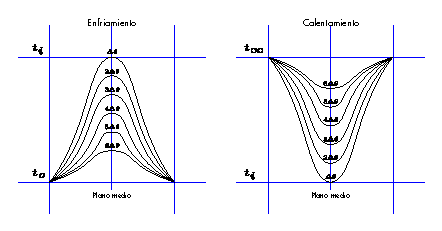
\includegraphics[scale=2.20]{figura03_09.eps}
\end{figure}

El método gráfico resuelve:
\begin{itemize}
    \item Problemas con $h=\infty$.
    \item Problemas con $h\ll\infty$.
    \item Problemas con temperaturas diferentes de las superficies externas.
\end{itemize}

El método de tabla numérica:
\begin{itemize}
    \item Problemas con $h=\infty$.
    \item Problemas con temperaturas diferentes de las superficies externas.
\end{itemize}

\section{Cuerpo semi-infinito}
Aquel cuerpo cuya dimensión mayor no se toma en cuenta en los cálculos, por
ejemplo: el suelo o una pared gruesa.
\begin{figure}[!h]
\centering
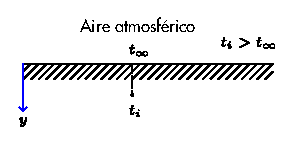
\includegraphics[scale=1.50]{figura03_10.eps}
\end{figure}

Para este caso se utiliza la ecuación de \emph{Fourier}:
\begin{equation*}
    \frac{\partial^2 t}{\partial y^2} =
    \frac{1}{\alpha}\frac{\partial t}{\partial\theta}
\end{equation*}

Además se cuentan con condiciones de contorno:
\begin{equation*}
    t(0,\theta)\rightarrow t = t_s
\end{equation*}
\begin{equation*}
    t(y,\theta)\rightarrow t = t_i
\end{equation*}

\subsection{Caso $h=\infty$}
\begin{equation*}
    \frac{t-t_s}{t_i-t_s} = \text{fer}\left(
        \frac{y}{\sqrt{4\alpha\theta}}
    \right)
\end{equation*}

Donde $t_s$ es $t_\infty$, es decir, la temperatura del medio fluido.
\begin{equation}
    \frac{t-t_\infty}{t_i-t_\infty} = \text{fer}\left(
        \frac{y}{\sqrt{4\alpha\theta}}
    \right)
\end{equation}

Donde:
\begin{itemize}
    \item $y$: Profundidad del plano.
    \item $t_i$: Temperatura del suelo.
    \item $t_\infty$: Temperatura del medio fluido (exterior).
    \item $t_s$: Temperatura de la superficie del suelo.
    \item $\text{fer}$: Función error.
\end{itemize}

La función error esta definida como:
\begin{equation}
    \text{fer}(\phi)=\frac{2}{\sqrt{\pi}}\int_0^{\phi} e^{-\eta^2} d\eta
    \label{error}
\end{equation}

\subsection{Caso $h\ll\infty$}
\begin{equation}
    \frac{t-t_i}{t_\infty-t_i} = 
    1 -
    \text{fer}(\xi) -
    \left[
        e^{\left(
            \frac{h\,y}{k}+\frac{h^2\alpha\theta}{k^2}
        \right)}
    \right]
    \left[
        1 - \text{fer}\left(
            \xi + \frac{h\sqrt{\alpha\theta}}{k}
        \right)
    \right]
\end{equation}

Donde:
\begin{equation}
    \xi = \frac{y}{\sqrt{4\alpha\theta}}
\end{equation}

\subsection{Calculo de la función error}
La función error puede calcularse de diferentes maneras:

\begin{description}
    \item [Método analítico] Se puede hallar valores calculando la integral de
        la ecuación (\ref{error}).
    \item [Método gráfico] Se puede hallar a partir de la gráfica de la
        función.
    \item [Tablas] Existen tablas para diferentes valores en el rango de $0$ a
        $2.5$, desde donde pueden ser interpolados valores intermedios.
\end{description}

